\documentclass{article}
\usepackage[utf8]{inputenc}
\usepackage[top=2cm,bottom=2cm, left=2cm, right=2cm]{geometry}

\usepackage{graphicx} %for figure formatting
\usepackage{float} %for figure formatting
\usepackage{fancyhdr} %for header and footer formatting
\usepackage{booktabs} %for table formatting
\usepackage{multirow} %for table formatting
\usepackage{multicol} %for multi column per page
\usepackage{siunitx} 
\usepackage{amsmath} %allow text in equation
\usepackage{amssymb} %allow symbols in equation
\usepackage{amsfonts}
\usepackage{changepage} %for adjusting width
\usepackage{gensymb} %To put in degree symbol
\usepackage{amssymb} %To put real number symbol
\usepackage{amsmath} %To align equations
\usepackage{mathtools}
\usepackage{braket} %To put put triangular brackets
\usepackage{esvect}
\usepackage{esint} %To put surface integrals
\usepackage{enumitem} %To change enumerate labels
\usepackage{physics} %To write PDEs
\usepackage{color,soul,multicol}
\usepackage{framed}
\usepackage[most]{tcolorbox}
\usepackage{xcolor}
\colorlet{shadecolor}{orange!15}
\usepackage[parfill]{parskip}
\setlength{\parskip}{1em}

\usepackage{hyperref}
\hypersetup{
    colorlinks,
    citecolor=black,
    filecolor=black,
    linkcolor=black,
    urlcolor=black
}



\title{BPES - Finance and Financial Management}
\author{Cooper}
\date{Spring Term 2023}

\begin{document}

\maketitle
\tableofcontents
\newpage

%%%%%%%%%% Main content %%%%%%%%%%

\section{Lecture 1: Introduction to Finance}
%% Lecture 1 19/01/2021
"qualitative in changing input on output, how the price would change." \par 
\begin{multicols}{2}
\subsection{Economics}
\boxed{\textbf{what is economics?}}
\begin{itemize}
    \item study of the production, distribution, and consumption of goods and services
    \item or can be interpreted as there's a lot of stuffs, how do you get stuffs to people
    \item focused on analysing behaviour and maximising welfare. (positive vs normative)
    \begin{itemize}
        \item positive analysis (factual): how do things work; normative: how should things work.
    \end{itemize}
    \item standard reasons for money:
    \begin{itemize}
        \item store of value: moving value through time. 
        \item medium of exchange: common goods for exchange
        \item unit of account: compare goods, one common denominator for comparison. 
    \end{itemize}
\end{itemize}

\boxed{\textbf{why economics paid attention with finance?}}\par
The financial problem blew up which also affects severely on the real economic, proving there're not unrelated but somehow intertwine, leading to \textit{macro-finance}

\subsection{Finance}
\boxed{\textbf{what is finance?}}
\begin{itemize}
    \item Finance is the study of investments. 
    \item The mean-variance approach (micro-level)
    \item The CAPM (macro-level)
    \item Two basic functions:
    \begin{itemize}
        \item Valuation: objective-independent, how are assets valued? How should they be valued?
    \end{itemize}
\end{itemize}

\subsubsection{Primary Market}
\textbf{primary market} is the financial market where entities such as companies, governments and other institutions obtain funds through the sale of debt and equity-based securities. selling part of the company and in return to share their profit.

\subsubsection{Secondary Market}

\textbf{secondary markets} is the financial market where investors buy and sell securities from other investors (stock exchange)

\subsubsection{Purpose of Financial Markets}

% first reason
\boxed{\textbf{why do we need financial market?}}\par
\begin{enumerate}
    \item Allows trading to offset and reduce risks (e.g. corn production with other investment, income is no longer unpredictable, as corn price might drop, profits from investing can save some downsides)
    \item (Setting Prices) The average aggregated information is reflected in the prices (more people want to sell, price goes down), which is valuable for people outside the market, companies, and policy makers. 
    \item (Transferring Risks) People expose to risk that doesn't want to be can have a place to sell it
\end{enumerate}
It essential for both group of these people (people with info vs people don't like risk) to make a financial market to function. 

\subsubsection{Important Assumptions}
\begin{enumerate}
    \item Agents are selfish
    \item Investors prefer more to less
    \item Investors don't like risk
    investors prefer money now to later
    \item No such thing as a free lunch, shouldn't allowed to create when nothing to start with 
    \item Financial market price to set supply = demand
    \item Risk sharing and frictions are central to financial innovation
    \item Don't say that a model is unrealistic. 
\end{enumerate}

\end{multicols}


\newpage
\section{Lecture 2: Time Value of Money }
Time value of money can be understood by expressing as a compensation for lack of liquidity (independent of the riskiness of what im investing) (risk-free), where
Assets can be formally defined as (1)\underline{\textbf{sequence of cashflows}}. And it is important to recall that (2)\underline{\textbf{One dollar today does not equal one dollar tomorrow}}

\begin{multicols}{2}

\subsection{Future Value (FV)}
\begin{gather*}
    \mathbf{FV = PV(1+RT)}
\end{gather*}

\subsection{Present Value (PV) or Price}
\begin{gather*}
    \mathbf{PV = \frac{FV}{(1+R)^T}}
\end{gather*}
       
\subsection{Yield (R): Rate of return}
\begin{gather*}
    \mathbf{R = \Big(\frac{FV}{PV}\Big)^{1/T}-1}
\end{gather*}

\subsection{Discount Factor}
\textbf{Discount factors} are how we value future cashflow, my willingness to buy and sell will depend on discount factor, how you convert future cashflow to today
\begin{itemize}
    \item (Risk-free) Discount factor for a period of t is:
    \begin{shaded}
        \begin{gather*}
            \mathbf{\frac{1}{(1+R)^t}}
        \end{gather*}
    \end{shaded}
    \item if my discount factor is \textbf{higher} than yours, that means I'm willing to \textbf{pay more} (higher PV) today than you are, i.e. willing to buy a bond from you. less risk averse (lower R)
    \item \textbf{lower} the discount factor, lower the patient you are willing to pay, and higher the the need for cash right now. \textbf{more risk averse} (higher R)
\end{itemize}

\subsection{Perpetuities}
How much is an infinite cashflow of C each year worth?
\begin{gather*}
    PV = \frac{C}{(1+R)}+\frac{C}{(1+r)^2}+\dots = \frac{C}{R}
\end{gather*}
\subsubsection{Growing/Infinite Perpetuities}
gets fixed amount of cash for a infinite number of periods. How much is an \textit{infinite} cash-flow of C growing at g each year worth?
\begin{gather*}
    \begin{split}
        &PV = \frac{C}{1+R}+\frac{C(1+g)}{(1+R)^2}+\frac{C(1+g)^2}{(1+R)^3}+\dots\\
        &PV = \frac{C}{R-g}
    \end{split}
\end{gather*}
\begin{itemize}
    \item for this to be well-defined, we need R $>$ g
    \item If g = R, that means g is perfectly compensating for my time value of money. i.e. All rhe growth in the payment getting are perfectly compensating me for the amount of time I'm losing, which indicates each cashflow is equally weighted for me.
    \item Effectively, this stream of infinite money is worth, in terms of how much I'm willing to pay is infinite amount of money. (value it infinitely because I'd be willing to pay infinitely amount), therefore there's NO well-defined price I can arrive to at for this.
\end{itemize}

\subsection{Fixed Horizon Annuities}
you get fixed amount of cash every period for a finite number of periods
How much is a fixed horizon cash-flow of C each year worth?
\begin{gather*}
    \begin{split}
        PV &= \frac{C}{(1+R)}+\frac{C}{(1+r)^2}+\dots+\frac{C}{(1+R)^T}\\
        (1+R)PV &= C + \frac{C}{1+R} + \dots + \frac{C}{(1+R)^{T-1}}\\
        RPV &= C - \frac{C}{(1+R)^T}\\
        PV &= \frac{C}{R} - \frac{C}{R(1+R)^T}\\
    \end{split}
\end{gather*}
T-period Annuity = Infinite Perpetuity - Date-T Perpetuity



\end{multicols}

\newpage
\section{Lecture 3: Portfolio Selection}
"The fundamental decision of investing is the allocation of your assets: How much should you own in stock? How much should you own in bonds? How much should you own in cash reserves"

\begin{multicols}{2}
    
\subsection{Expected Value}
Suppose that a return $R_i$ on asset i is equal to $R_i(s)$ in state s. And that states'
probabilities of occurrence are given by p(s), for s = 1, ..., S.
\begin{gather*}
    E[R_i] = \sum_{s=1}^{S}R_i(s)p(s)
\end{gather*}

\subsection{Variance}
The volatility or risk of $R_i$ is often refer to the \textbf{standard deviation} $\sigma_i$ (will be redefined later)
\begin{gather*}
    \begin{split}
        Var[R_i] &= \sigma_i^2 = E[(R_i(s)-E[R_i])^2]\\
        &= \sum_{s=1}^{S}p(s)(R_i(s)-E[R_i])^2
    \end{split}
\end{gather*}

\subsection{Covariance}
The degree of two assets in a portfolio move in the same direction at the same time.
\begin{gather*}
    Cov(R_i,R_j) = \sum_{s=1}^{S}p(s)(R_i(s)-E[R_i])(R_j(s)-E[R_j])\\
    Var[wA+vB] = w^2Var[A]+v^2Var[B] + 2wvCov[A,B]
\end{gather*}

\subsection{Correlation}
Measure the strength and direction two assets in a portfolio moves at the same time. 
\begin{gather*}
    Corr(R_i,R_j) = \rho_{ij}=\frac{Cov(R_i,R_j)}{\sigma_i\sigma_j}
\end{gather*}

\subsection{Portfolio Allocation}
\subsubsection{1 risky, 1 risk-free}
\underline{\textbf{Risk-free asset:}}\\
A baseline to compare with risky assets. normally deemed as the US Treasury Bill (not true this year). 
\begin{gather*}
    E[R_f] = R_f,\hspace*{0.3cm}V[R_f] = 0,\hspace*{0.3cm}Cov[R_f] = 0
\end{gather*}
The expected return for this kind of portfolio can be express as,
\begin{gather*}
    \begin{split}
        E[R_p] &= E[wR_i+(1-w)R_f]\\
        &= \boxed{R_f+w\overbrace{E[\underbrace{R_i-R_f}_\text{excess return}]}^\text{risk premium}}
    \end{split}
\end{gather*}
and the variance of the portfolio will be 
\begin{gather*}
    \begin{split}
       V[R_p] &= V[wR_i+(1-w)R_f]= w^2\sigma_i^2\\
        \sigma_p &= \lvert w\rvert\sigma_i
    \end{split}
\end{gather*}
\underline{\textbf{The Captial allocation line:}}\\
substituting the above, we can re-express expected value as the following, this is also know as the Capital Allocation Line, where the only possible combination of 1 risky and 1 risk-free lies on this line. What the investor \textit{can} get.
\begin{gather*}
    E[R_p] = R_f+wE[R_i-R_f] = R_f+\underbrace{\frac{E[R_i-R_f]}{\sigma_i}}_\text{Sharpe ratio}\sigma_p
\end{gather*}
\underline{\textbf{Indifference Curve:}}\\
Indifference curves expresses sets of portfolios that would make investors equally happy, they must slope upwards, and it also increases value from left to right. Indifference curves represent what investors want. If risk-neutral, Indifference curves becomes straight lines.

\underline{\textbf{Utility Function:}}\\
uses mean-variance utility to measure how risk tolerant and risk averse investor will value stocks
\begin{gather*}
    E[U(R_p)] = E(R_p)-0.5A\cdot V(R_p)
\end{gather*}
$A$ is a measure of risk aversion, the bigger the A is, the more risk averse the investor is. 

\subsubsection{2 risky, 1 risk-free}
\begin{figure}[H]
    \centering
    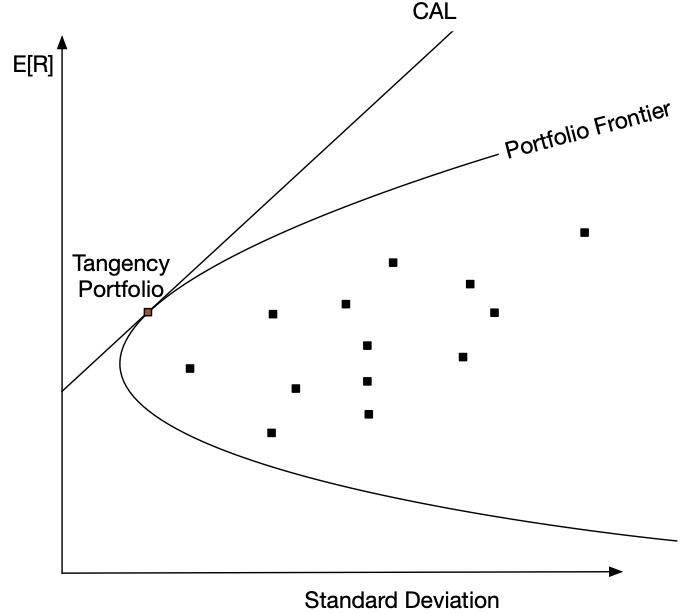
\includegraphics[width =0.3\textwidth]{Figure/cal.png}
\end{figure}
\subsubsection{Equal-Weighted Portfolio}
Equally weighted portfolio of independent assets. $Cov(R_i,R_j)=0$, variance of the portfolio then becomes, 
\begin{gather*}
    \sigma_p^2 = \frac{1}{N}\sum_{i=1}^{N}\sigma_i^2 = \frac{1}{N}E[\sigma_i^2]
\end{gather*}
Risk decreases with the number of assets. Standard deviation declines with the number of assets.


\end{multicols}

\newpage
\section{Lecture 4: Capital Asset Pricing Model (CAPM)}
Now we need to find a way to quantify risk, especially systemic risk (idiosyncratic risk can be diversified away), of an asset or an asset in our portfolio. 

\begin{multicols}{2}
    
In the CAPM framework, all investors are assumed to have access to the same information and hold homogeneous expectations about future returns, and the market portfolio is considered to be the only efficient portfolio, meaning that it offers the highest expected return for a given level of risk.\par 

Then we can effectively transfer our original Tangency Portfolio into our \underline{\textbf{Market portfolio}}, and our capital allocation line (CAL) into \underline{\textbf{Capital Market Line}}, the line that connects the Market Portfolio to the risk-free rate
\begin{figure}[H]
    \centering 
    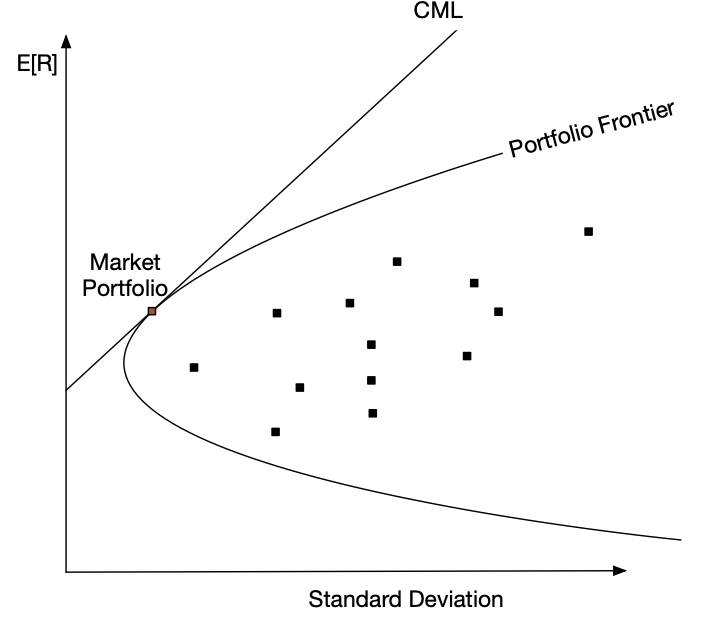
\includegraphics[width =0.4\textwidth]{Figure/cml.png}
\end{figure}
Given the assumption, the risk-reward ratio of any asset or portfolio is determined solely by its beta, and the expected return for each unit of systematic risk should be the same for all assets and portfolios. 
\begin{gather*}
    \frac{E[R_i]-R_f}{Cov[R_M, R_i]} = \frac{E[R_M]-R_f}{V[R_M]}\\[0.1cm]
    E[R_i] = (E[R_M]-R_f)\frac{Cov(R_M,R_i)}{V[R_M]}+R_f\\
    \boxed{E[R_i] =  R_f + \beta(E[R_M]-R_f)}
\end{gather*}
$\beta$ is therefore the measure of systemic risk of an asset. This is because according to CAPM in an efficient market, investors are only compensated for bearing systematic risk, which is the risk that cannot be diversified away by holding a diversified portfolio.

\subsection{Application of CAPM (1) -- Excess Return}
Analyst compare stocks' returns with their fair expected return from the CAPM
\begin{gather*}
    \alpha = E[R_i]-[R_f+\beta(E[R_M]-R_f)]
\end{gather*}
A stock's $\alpha$ is the unexpected deviation from the fair return. Stocks with high alpha are under-valued and should be bought.

\subsection{Application of CAPM (2) -- Capital Budgeting Decisions}
CAPM can also be used to judge whether firms should undertake risky projects. This can be done by calculating the Net Present Value (NPV) or compare the CAPM expected return with internal rate of return (IRR) (the rate of return where NPV = 0). If $E[R_i]>IRR$, then the firm should reject the project. 

\subsection{Index Model}
An index model uses an actual stock index to proxy this theoretical market. CAPM makes forward-looking predictions. Index models use historical data. Index model states that
\begin{gather*}
    R_i-R_f = \alpha_i+\beta_i[R_M-R_f]+\varepsilon_i
\end{gather*} 
$\alpha$ is the abnormal return and $\varepsilon$ is the firm specific risk, which is idiosyncratic risk. And the CAPM equation can be rewritten in terms of the index model
\begin{gather*}
    \boxed{R_i = R_f+\beta_i[R_M-R_f]+\varepsilon_i}
\end{gather*}
The variance percentage of the idiosyncratic risk and systemic risk can therefore be quantify as 
\begin{gather*}
    \begin{split}
        V[R_i] &= V[R_f+\beta_i[R_M-R_f]+\varepsilon_i]\\
        \sigma_i^2 &= V[\beta_i(R_M-R_i)+\varepsilon_i]\\
        &= \beta_i\sigma_M^2 + \bar{\sigma_i}^2
    \end{split}
\end{gather*}
$\boxed{\bar{\sigma_i}^2/\sigma_i^2}$ is the variance percentage that is \textbf{idiosyncratic} and 1-term will then be the systemic risk








\end{multicols}

\newpage
\section{Lecture 5: Risk Pricing and Arbitrage}
Arbitrage is a trading strategy that \textbf{(1)} require NO initial investment. \textbf{(2)} Has \underline{NO negative cash flows} at any time. \textbf{(3)} Has a positive cash flow at at least one time. Arbitrage also implies and solves mispricing. 

\begin{multicols}{2}
Important insight in theoretical finance: (1) True arbitrage cannot exist. (2) Prices would adjust to eliminate it. (3) The no-arbitrage condition.

\subsection{Bid-Ask Spread}
\underline{\textbf{Bid:}} the price at which market maker buys an asset.\\[0.2cm]
\underline{\textbf{Ask:}} the price at which market maker sells an asset.\\[0.2cm]
\underline{\textbf{Mid:}} (Bid+Ask)/2, a way to value holdings.\par 
\underline{The Bid-Ask spread} is normally set base on liquidity and other reasons, for a market maker, they care about (1) Their risk aversion (2) Internal guidelines on inventory (3) Reputations. (4) \textbf{Adverse Selection}. if an investor wished to purchase stocks from a fund and has inside or more research on that specific asset, them the fund might widen their spread to minimise their risk in order to offset this lack of information.

\subsection{Implication of No Arbitrage}
\subsubsection{The Law of One Price (LOOP)}
If two securities have the same payoffs, they have the same price. e.g.\par 

Chase is offering a bond that pays \$100 in one year, at \$94.34.
Merrill Lynch is offering a bond that pays \$100 in one year, at \$95.23. In this arbitrage example, arbitrageurs tends to borrow/sell Merrill Lynch bond and buy the Chase bond to make profit.However transaction costs make it more difficult to find arbitrages, there isn't necessarily a deterministic price with transaction costs.

\subsubsection{Replicating Portfolio}
If a portfolio has the same payoffs as a security, it must have the same price. e.g.\par

If a bond three-year bond with a 10\% coupon rate is trading for \$100. At the same time 
\begin{itemize}
    \item A zero-coupon bond maturing in 1 year costs \$98
    \item A zero-coupon bond maturing in 2 year costs \$96
    \item A zero-coupon bond maturing in 3 year costs \$93
\end{itemize}

From the replicating portfolio, we can refer that \$10 in \underline{one year} is worth \$9.8 today; \$10 in \underline{two year} is worth \$9.6 today, \$110 in \underline{three year} is worth \$102.3 today, the bond should worth \textcolor{red}{\$121.7}, therefore, buy the bond and short the replicating portfolio if it's priced at \$100.

\subsubsection{Dynamic Hedging Strategy}
If a self-financing strategy has the same payoffs as a security, it must have the same price. e.g.\par 

How much should a zero-coupon bond maturing in two years cost if:
\begin{itemize}
    \item A zero-coupon bond maturing in one year costs \$98.
    \item In one year, a one year zero-coupon bond also costs \$98.
\end{itemize}
Need \$100 in two year, so i need \$98 in one year (for the second point), therefore, to get only \$98 in one year, the bond today will cost 0.98*98= \$96.04. If priced at \$95: buy the two-year zero. Short 0.98 units of the 1-year zero at \$96.04. Make \$1.04.

\end{multicols}

\newpage
\section{Lecture 6: Equity Valuation}
This section will be discussing on the intrinsic value and market of an equity, particularly on stocks 

\begin{multicols}{2}
    
\subsection{intrinsic Value}
Value $V$ based on a fundamental analysis of a company's current assets and future prospects. It is the discounted value of the cash that can be taken out of a business during its remaining life. 

\subsection{Market Value}
Value $P$ based on observed market prices and shares outstanding.

\subsection{Dividend Discount Model (DDM)}
Equity's value is equal to the discounted value of all future dividends.
\begin{gather*}
    \begin{split}
        V_0 = P_0 &= \frac{E(D_1)}{1+R}+\frac{E(P_1)}{1+R}\\
        &= \frac{E(D_1)}{1+R} + \frac{E(\frac{E(D_2)}{1+R}+\frac{E(P_2)}{1+R})}{1+R}\\
        &= \frac{E(D_1)}{1+R}+\frac{E(D_2)+E(P_2)}{(1+R)^2}\\
        &= \frac{E(D_1)}{1+R} + \frac{E(D_2)}{(1+R)^2} + \frac{E(D_3)}{(1+R)^3} + \cdots
    \end{split}
\end{gather*}
In order to price a equity from its dividends, we first need to find out how to evaluate a company's dividend.

\subsection{Expected Dividend}
\subsubsection{Dividend Payout Ratio}
Ratio $d$ is equal to the expected share of earnings that will be paid out as a \underline{\textbf{dividend}}.
\begin{gather*}
    \boxed{D_t = d_t\times E_t}
\end{gather*}

\subsubsection{Earnings-Retention Ratio}
Ratio $b$ is equal to the expected share of earnings that will be \underline{\textbf{reinvested}}.
\begin{gather*}
    I_t = b_t\times E_t = (1-d_t)E_t
\end{gather*}
if the retained earnings fund new projects with return $ri$. the expected return can then expressed as
\begin{gather*}
    E_{t+1} = E_t + I_t\times ri_{t+1} = E_t+b_t\times E_t\times ri_{t+1}\\
    \boxed{g_{t+1}=\frac{E_{t+1}-E_t}{E_t} = b_t\times ri_{t+1}}
\end{gather*}
This leads to The \underline{\textbf{Growth Rate of Earnings}}:

\subsection{DDM Analysis}
\subsubsection{D constant}
Suppose that the dividends are \underline{\textbf{constant}}, i.e. $E(D_1) = D_0, E(D_2) = D_0...$
\begin{gather*}
    \begin{split}
        V_0 &= \frac{E(D_1)}{1+R} + \frac{E(D_2)}{(1+R)^2}+\cdots\\
        &= \frac{D_0}{1+R} + \frac{D_0}{(1+R)^2}+\cdots = \boxed{\frac{D_0}{R}}
    \end{split}
\end{gather*}
\subsubsection{D grow at rate g}
Suppose now the \underline{\textbf{dividends grow}} at a rate g, i.e. $E(D_1) = (1+g)D_0$, $E(D_2) = (1+g)^2D_0$
\begin{gather*}
    \begin{split}
        V_0 &= \frac{D_0(1+g)}{1+R}+\frac{D_0(1+g)^2}{(1+R)^2}+\cdots\\
        &= \frac{D_0(1+g)}{R-g} = \boxed{\frac{(1-b)E(E_1)}{R-g}}
    \end{split}
\end{gather*}
This is also called the \underline{\textbf{Gordon Growth Model}}\par 

From the table below, the amount of investment increases from left to right, and price adjust accordingly. If the return on new investment is exactly $\boxed{\textbf{equal}}$ to the \textcolor{red}{\textbf{CAPM implied return}}, the things I'm investing in are compensating me exactly as well as the stock should be compensating me, so the price will remain unchanged\par 

If the new investment return is $\boxed{\textbf{lower}}$ than my CAPM implied return, that means I'm investing into something bad that doesn't gives me enough return, therefore, the \underline{\textbf{stock price must decrease}} in order to \textbf{increase} the expected return. 

Likewise, if my new investment return is $\boxed{\textbf{higher}}$ than my CAPM implied return, than the stock \underline{\textbf{price must increase}} in order to \textbf{decrease} the expected return.\footnote{a stock with a very high price will require a larger dollar change in price to achieve the same percentage return as a stock with a very low price, resulting in a lower percentage return for the higher-priced stock. E.g. Stock A is priced at \$500 per share and Stock B is priced at \$50 per share. If both stocks increase in price by \$50 per share over a period of time, Stock A would have a 10\% return (\$50 / \$500), while Stock B would have a 100\% return (\$50 / \$50)}


\subsection{Two stage valuation}
If a company dividends grow at different rates over time, i.e. first stage at rate $g_1$, second stage $g_2$ 
\begin{gather*}
    V_0 = \sum_{t =1}^{T}\frac{D_0(1+g_1)^t}{(1+R)^t} + \frac{D_T(1+g_2)}{(R-g_2)(1+R)^T}
\end{gather*}

\subsection{Valuation Ratio}
\subsubsection{Price-dividend ratio}
\begin{gather*}
    \frac{P}{D} = \frac{1+g}{R-g}
\end{gather*}

\subsubsection{Price-earnings ratio}
\begin{gather*}
    \frac{P}{E} = \frac{(1+g)(1-b)}{R-g}
\end{gather*}

\end{multicols}

\begin{figure}[H]
    \centering 
    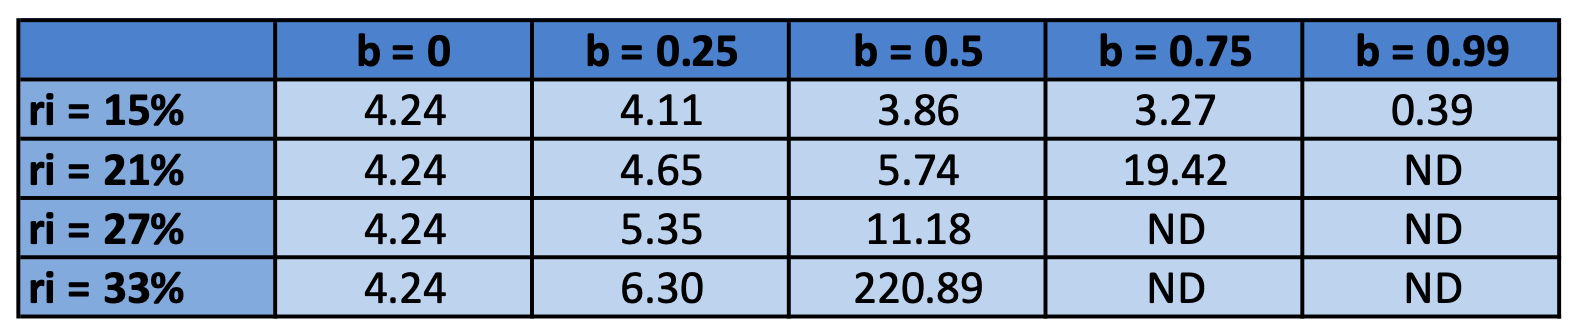
\includegraphics[width =0.7\textwidth]{Figure/table.png}
\end{figure}




\newpage
\section{Lecture 7: Fixed Income Valuation}
\begin{multicols}{2}
    

\subsection{Bond Pricing}
$V_0$ is the current value of the bond (at time 0). $C_t$ is the coupon payment at time $t$. $FV_T$ is the face value at maturity. $r_{0,t}$ is the current interest rate for investment maturing at time T. 
\begin{gather*}
    V_0 = \sum_{t=1}^{T}\frac{C_t}{(1+r_{0,t})^t}+\frac{FV_T}{(1+r_{0,T})^T}
\end{gather*}

\subsection{Yield To Maturity (YTM)}
\begin{itemize}
    \item Yield to maturity (YTM) is the total return anticipated on a bond if the bond is held until it matures, accounting for the present value of a bond's future coupon payments
    \item Yield to maturity is the total rate of return that will have been earned by a bond when it makes all interest payments and repays the original principal.
    \item YTM is essentially a bond's internal rate of return (IRR) if held to maturity.
\end{itemize}
Given a price $P_0$, the the yield to maturity is the discount rate $y$ that sets the value $V_0$ equal to the price:
\begin{gather*}
    y\hspace*{0.3cm}s.t.\hspace*{0.3cm}P_0 = \sum_{t=1}^{T}\frac{C_t}{(1+y)^t}+\frac{FV_T}{(1+y)^T}
\end{gather*}
 
\subsection{Forward Interest Rate}
The forward rate is the \textit{inferred} rate from the yield curve. Say we have spot interest rate for investments with a one-year maturity, \underline{$r_{0,1}$ = 0.26\%}. and spot interest rate for a two-year maturity, \underline{$r_{0,2}$ = 0.68\%}, what would the Forward interest rate for one year investments starting in one year, $f_{1,2}$ be?
\begin{gather*}
    (1+r_{0,2})^2 = (1+r_{0,1})(1+f_{1,2})
\end{gather*}
This can be express as the \textbf{(1)} two year maturity value must equal to the one year maturity + the forward rate value due to arbitrage limitation. we can also be inferred that the \textbf{(2)} two year bond interest rate will be an average of the combination of the one year + forward interest rate. Thus, for an upward slopping yield curve, the \textbf{forward interest rate must be higher than both the one year and the two year} 

\subsection{Monetary Policy (Central Bank)}
Purpose of messing with money supply: (1) Control inflation (2) low and sustainable unemployment. \par
\textbf{Inflation:}
\begin{itemize}
    \item need to raise interest rate $\rightarrow$ take money out of circulation(market) $\rightarrow$ sell lots of government bond $\rightarrow$ bond price drops 
    $\rightarrow$ increases interest rate and yield 
    \item people tends to other use of money to get better profits (i.e. save in the bank), thus, bond prices tend to drop to attract.
    \item When \textcolor{red}{\textbf{interest rates rise}}, existing bonds paying lower interest rates become less attractive, causing their \textcolor{red}{\textbf{price to drop}} below their initial par value in the secondary market. (The coupon payments remain unaffected.) \textcolor{red}{\textbf{also increases the yield}}
    
\end{itemize}
\textbf{Recession:}
\begin{itemize}
    \item need to lower interest rate $\rightarrow$ put money into circulation(market) $\rightarrow$ buy lots of government bond $\rightarrow$ bond price increases (supply drops) $\rightarrow$ decreases interest rate and yield 
\end{itemize}

\subsection{Expectations Theory}
\textbf{(1)} Long run rates are a geometric average of current and future short rates. \textbf{(2)} The expected future interest rate is equal to the forward rate.
\begin{gather*}
    (1+r_{0,2})^2 = (1+r_{0,1})(1+E[r_{1,2}])
\end{gather*}
Empirically, slope of yield curve is good predictor of GDP growth rate (recession)

\subsection{Liquidity Preference Theory}
\textbf{(1)} Long-term lenders require compensation due to lack of liquidity ($\pi_{1,2}$ liquidity premium). \textbf{(2)} higher yields for longer maturity bonds, the yield curve will then be upwards slopping independent of the expectations. 
\begin{gather*}
    (1+r_{0,2})^2 = (1+r_{0,1})(1+E[r_{1,2}]+\pi_{1,2})
\end{gather*}
If the yield curve is observed to be \textcolor{red}{upwards sloping}, then future spot rates are expected to be \textcolor{red}{higher than current} spot rates under \underline{Rational Expectations} Theory and \textcolor{red}{indeterminate} under \underline{Liquidity Preference} Theory
\subsection{Segmented Markets Theory}
different people are trading different stuffs, thus you can't do much interference on comparing markets. e.g. index tax funds wants to hold the longest safest bonds possible (30 years), bond price increases, yield decreases. This explains persistent differences in rates (20yr vs 30yr). They trade it because they "like" it.

\subsection{Duration}
Bond prices may be affected severely to interest rate risk, how much will the bond price be affected by changes in interest rate? What happens when the \textbf{yield curve shifts up parallel (level).}
\begin{gather*}
    D = -\frac{dP}{dy}\frac{1+y}{P} = \sum_{t=1}^{T}w_tt\hspace*{0.4cm}\text{where}\hspace*{0.2cm}w_t = \frac{\text{CashFlow}_t}{P(1+y)^t}
\end{gather*}
\begin{itemize}
    \item Duration can measure how long it takes, in years, for an investor to be repaid a bond's price by the bond's total cash flows
    \item Duration also measures a bond's or fixed income portfolio's price sensitivity to interest rate changes.
    \item Most often, when \textcolor{red}{interest rates rise}, the higher a bond's duration, the more its price will fall.
    \item Higher Duration $\rightarrow$ lower coupon rate (longer term to maturity and more volatility) $\rightarrow$ more vulnerable to interest rate risk
    \item Higher coupon has the shorter duration. 
    \item e.g. for duration of 5 years, 1\% increase in interest rate, bond value decreases by 5\%, vice versa.
    \item Sharpeners and levellers are strategies to \textbf{hedge yield curve shape} changing. 
\end{itemize}


\end{multicols}

\newpage
\section{Lecture 8: Options}
Contracts that give one party the \textbf{(1)} \textit{right} to buy or sell a certain security, target risk better and information. \textbf{(2)} Allow us to learn incredibly granular levels of information. \textbf{(3)} target risks better and incredibly specific \textbf{(4)} Put information in a more targeted way. 





%%%%%%%%%% %%%%%%%%%%



\end{document}
